\section{Dataset and Features}
\subsection{Dataset Generation}
\label{sec:dandf}
\begin{figure}[H]
\centering
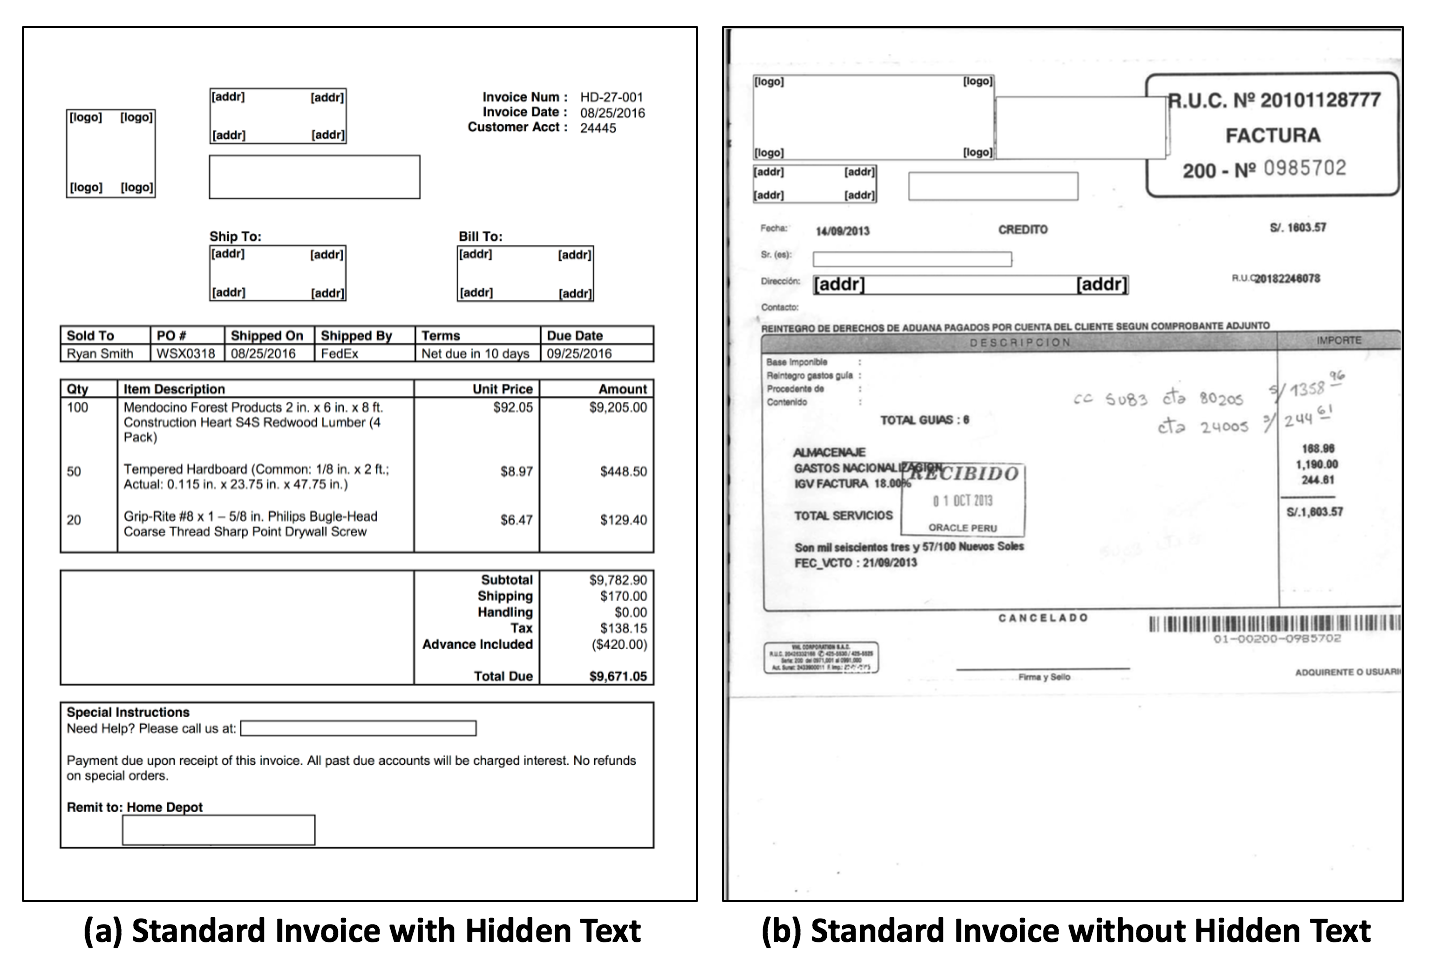
\includegraphics[width=1\linewidth]{invoiceexp.png}
\caption{Sample Invoices}
\label{fig:invoiceexp}
\end{figure}
% \begin{figure}[H]
% \centering
% 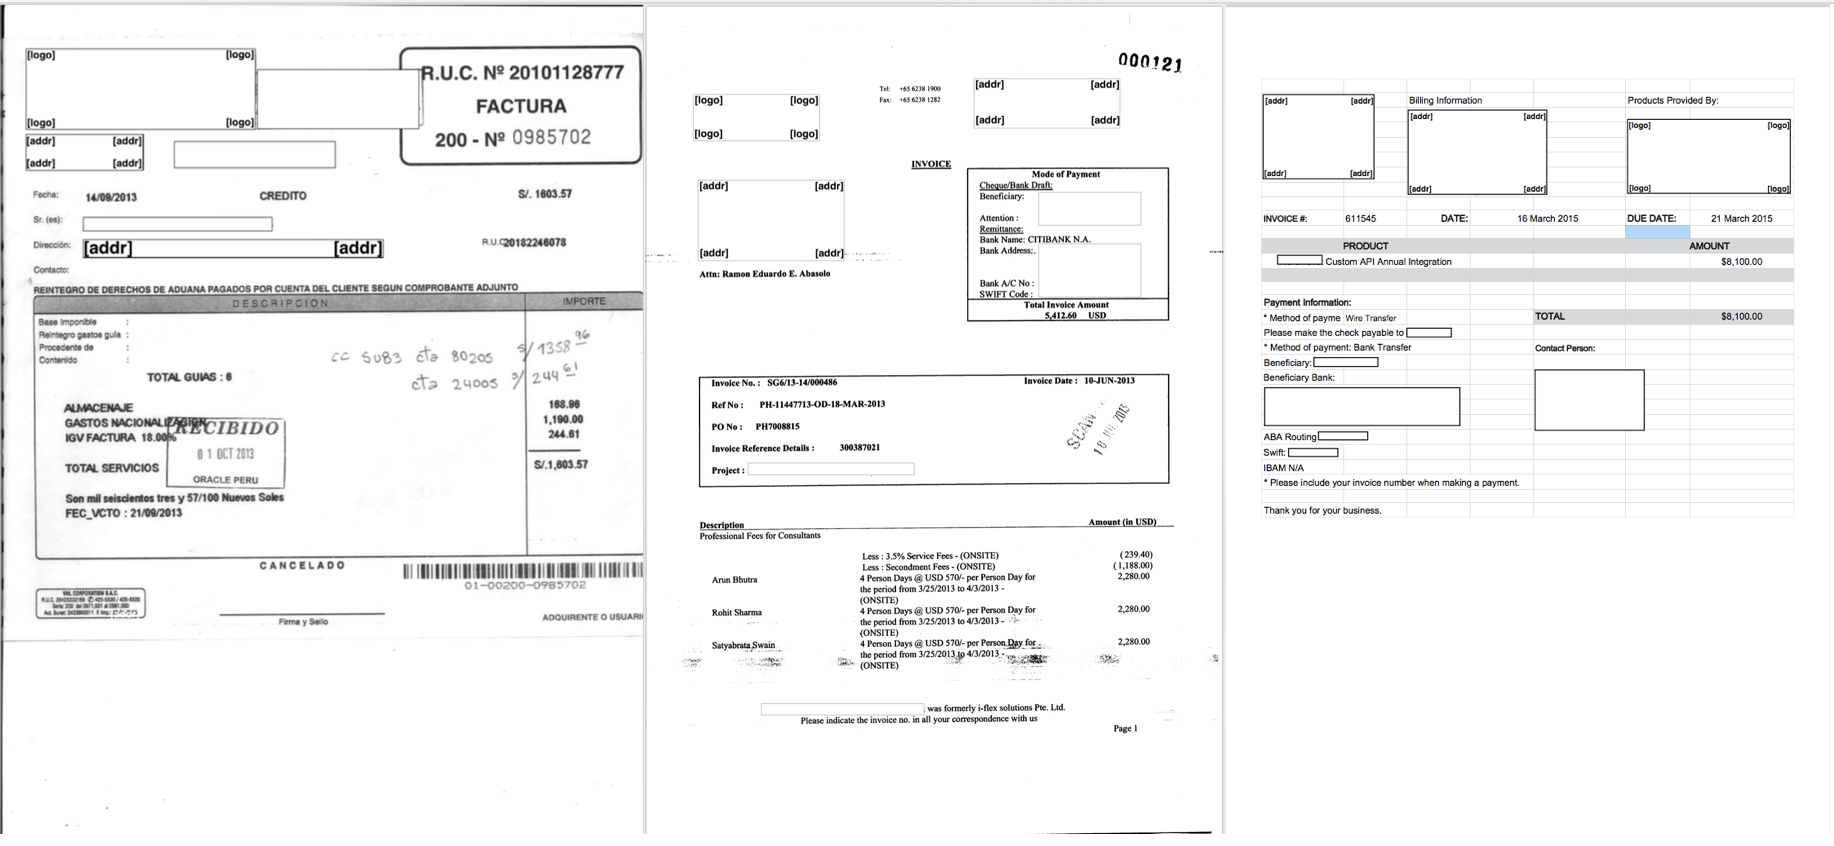
\includegraphics[width=1\linewidth]{nonstandardinvoice.png}
% \caption{Sample Non-standard Invoice without hidden text}
% \label{fig:nonstandardinvoice}
% \end{figure}

97 raw invoice images are obtained from the internal testing library of Oracle Corporation, examples of which are displayed in Fig. \ref{fig:invoiceexp}. Sensitive information has been manually replaced with tokens (LOGO, ADDR, etc) labeled on the corners of the bounding boxes, to preserve position without revealing the actual text. While some are well-formatted PDF files with hidden text, most are TIFF images that require additional steps before PDF Layout Analysis\cite{shinyamapdfminer} can take place to extract word groups. The process of generating word groups and coordinates as actual training input is outlined  in Fig. \ref{fig:flow2}

TIFF images are first rotated to best alignment with rotation angle calculated from Hough Line Transform\cite{vc1962method}, and then performed Optical Character Recognition (OCR)\cite{smith2007overview} to obtain any textual groups exist in the image. All sample invoices are then sent to PDF Layout Analysis, where coordinates of tokenized textual groups are retrieved and stored. Then, additional word processing is implemented on each token, including Porter2 word stemming\cite{stemming}, stopwords removal\cite{loper205028nltk}, and type identification using regular expressions. 5 special types - DATE, MONEY, NUMBER, TELE, and EMAIL - are defined for the last process, where the exact textual values are substituted for more generic representation.

\subsection{Feature Generation}
For each token, the following set of feature selection rules is applied: horizontally aligned tokens, vertically aligned tokens, nearby tokens within a distance threshold, overall vertical position, and its own type. The resulting features from each token are then accumulated to form the bag of potential features, where binary values are used to track whether any given feature exists for a token. For instance, if token $A$ is horizontally aligned with token $B$, feature $B\_halign$ will be generated and be of value $1$ for $A$ and 0 otherwise. The feature selection rules are picked to capture basic layout information, without presumption of any standard template.

Around 8000 features were generated for the 2095 tokens ($m=2095$) in 97 invoices, and further reduced through preliminary feature pruning
(Section~\ref{sec:dandf}) to exclude the ones that only appear once (and are thus not indicative). The remaining features ($n\approx2000$) are then put into careful feature selection process detailed in Section $V$.